\documentclass[10pt, a5paper]{article}
\usepackage{pdfpages}
\usepackage{parallel}
\usepackage[T2A]{fontenc}
\usepackage{ucs}
\usepackage[utf8x]{inputenc}
\usepackage[polish,english,russian]{babel}
\usepackage{hyperref}
\usepackage{rotating}
\usepackage[inner=2cm,top=1.8cm,outer=2cm,bottom=2.3cm,nohead]{geometry}
\usepackage{listings}
\usepackage{graphicx}
\usepackage{wrapfig}
\usepackage{longtable}
\usepackage{indentfirst}
\usepackage{array}
\newcolumntype{P}[1]{>{\raggedright\arraybackslash}p{#1}}
\frenchspacing
\usepackage{fixltx2e} %text sub- and superscripts
\usepackage{icomma} % коскі ў матэматычным рэжыме
\PreloadUnicodePage{4}

\newcommand{\longpage}{\enlargethispage{\baselineskip}}
\newcommand{\shortpage}{\enlargethispage{-\baselineskip}}

\def\switchlang#1{\expandafter\csname switchlang#1\endcsname}
\def\switchlangbe{
\let\saverefname=\refname%
\def\refname{Літаратура}%
\def\figurename{Іл.}%
}
\def\switchlangen{
\let\saverefname=\refname%
\def\refname{References}%
\def\figurename{Fig.}%
}
\def\switchlangru{
\let\saverefname=\refname%
\let\savefigurename=\figurename%
\def\refname{Литература}%
\def\figurename{Рис.}%
}

\hyphenation{admi-ni-stra-tive}
\hyphenation{ex-pe-ri-ence}
\hyphenation{fle-xi-bi-li-ty}
\hyphenation{Py-thon}
\hyphenation{ma-the-ma-ti-cal}
\hyphenation{re-ported}
\hyphenation{imp-le-menta-tions}
\hyphenation{pro-vides}
\hyphenation{en-gi-neering}
\hyphenation{com-pa-ti-bi-li-ty}
\hyphenation{im-pos-sible}
\hyphenation{desk-top}
\hyphenation{elec-tro-nic}
\hyphenation{com-pa-ny}
\hyphenation{de-ve-lop-ment}
\hyphenation{de-ve-loping}
\hyphenation{de-ve-lop}
\hyphenation{da-ta-ba-se}
\hyphenation{plat-forms}
\hyphenation{or-ga-ni-za-tion}
\hyphenation{pro-gramming}
\hyphenation{in-stru-ments}
\hyphenation{Li-nux}
\hyphenation{sour-ce}
\hyphenation{en-vi-ron-ment}
\hyphenation{Te-le-pathy}
\hyphenation{Li-nux-ov-ka}
\hyphenation{Open-BSD}
\hyphenation{Free-BSD}
\hyphenation{men-ti-on-ed}
\hyphenation{app-li-ca-tion}

\def\progref!#1!{\texttt{#1}}
\renewcommand{\arraystretch}{2} %Іначай формулы ў матрыцы зліпаюцца з лініямі
\usepackage{array}

\def\interview #1 (#2), #3, #4, #5\par{

\section[#1, #3, #4]{#1 -- #3, #4}
\def\qname{LVEE}
\def\aname{#1}
\def\q ##1\par{{\noindent \bf \qname: ##1 }\par}
\def\a{{\noindent \bf \aname: } \def\qname{L}\def\aname{#2}}
}

\def\interview* #1 (#2), #3, #4, #5\par{

\section*{#1\\{\small\rm #3, #4. #5}}

\def\qname{LVEE}
\def\aname{#1}
\def\q ##1\par{{\noindent \bf \qname: ##1 }\par}
\def\a{{\noindent \bf \aname: } \def\qname{L}\def\aname{#2}}
}

\begin{document}
\title{Модуль инструментальной оценки состояния пользователя}
\author{Латий О.О., Костюк Д.А., Брест, Беларусь\footnote{\url{denis_pynkin@epam.com}, \url{http://lvee.org/en/abstracts/168}}}
\maketitle
\begin{abstract}
An open hardware project to measure physical state changes of the user while his/her interaction with software is presented. Galvanic skin response, heart rate and blood pressure are used as measured parameters. A schematics is proposed to get these parameters from electric and optical sensors. Arduino platform is engaged in getting data from developed sensors and passing them via USB cable to the receiving software, to store log in CSV format.
\end{abstract}
\subsection*{Введение}

Измерение физического состояния пользователя при работе с программным обеспечением позволяет определить «узкие места» интерфейса гораздо эффективнее, чем такие более типичные методы, как опросы пользователей или составление тестовых заданий и экспертный анализ их выполнения. Более того, для результатов, выдаваемых измерительным устройством, легко выполнить качественное сравнение в разных исходных условиях (графических оболочках, офисных пакетах и др.), не полагаясь на квалификацию usability-эксперта.  Как следствие, инструментальная оценка позволяет быстро сформировать набор предложений по улучшению ПО.

Ниже нами представлен разработанный на принципах open \linebreak hardware аппаратный проект, позволяющий эффективно выполнять такую оценку. Разработка доступна по адресу \url{https://github.com/fiowro/uxdump}.

\subsection*{Измеряемые параметры}

Представляемый здесь модуль одновременно оценивает три параметра: электрическую проводимость кожи (ЭПК), сердечный \linebreak ритм и относительное изменение кровяного давления.

ЭПК варьируется в зависимости от влажности кожи, которая обеспечивается потовыми железами, контролируемыми симпатической нервной системой \cite{bib1, bib2}. По этой причине электропроводность часто используется как показатель психологического или физиологического возбуждения. Однако на результаты измерений ЭПК заметно влияют как внешние факторы (температура, влажность), так и внутренние (воздействие принятых медикаментов). По этой причине измерения ЭПК обычно используются совместно с регистрацией других показателей: сердечного ритма, ритма дыхания, кровяного давления и др. Очевидно, что легче всего регистрировать среди перечисленных параметров сердечный ритм.

При физической нагрузке, изменении эмоционального состояния, а также под воздействием иных факторов частота сердечных сокращений (ЧСС) увеличивается, так как организм человека реагирует на требование органам и тканям повышенного кровоснабжения увеличением сердечных сокращений. Кровяное давление, в свою очередь, является одним из главных показателей здоровья человека, и также известно как индикатор стрессового состояния.

Определение ЭПК, как электрической характеристики --- технически простая задача. Есть также несколько несложных способов автоматического определения ЧСС. Наиболее простой в реализации способ основан на принципе фотоплетизмографии (ФПГ), когда информация об изменении объема крови в тканях считывается оптическим методом. Фотоплетизмограф недостаточно точен для получения абсолютной величины объема, но позволяет четко отслеживать его относительные изменения, и потому хорошо подходит для определения интервалов времени.

Похожим способом, по методу определения времени распространения пульсовой волны (ВРП), может быть оценено относительное изменение давления (авторы благодарят Юрия Адамова за указание на данный метод). ВРП обычно определяется как время, затрачиваемое кровью для преодоления расстояния от сердца, с момента ее выброса, до какой-либо точки, обычно пальца. Зная время задержки между пиками на графиках пульса или скорость нарастания пульса, можно оценить изменение кровяного давления.

Описанные принципы измерения доступны для реализации в относительно несложных устройствах, что и послужило побудительным мотивом для создания представленной разработки.

\subsection*{Аппаратная платформа и особенности реализации}

В качестве основы для измерительных модулей нами выбрана платформа Arduino \cite{bib2}. Программирование и обмен данными с ПК выполняется через USB-обертку последовательного интерфейса.

Схема разработанного нами измерительного блока, расширяющего платформу Arduino для совместного измерения ЭПК и ЧСС представлена на  рисунке \ref{latij1} (с поправкой на то, что для оценки изменений давления реальное устройство включает не один, а два блока измерения ЧСС). Элементы схемы включают обеспечение электрического смещения ИК-диода, соответствующее электрическое смещение фотодиода, ВЧ-фильтрацию для удаления низкочастотных артефактов движения и дребезга, а также НЧ-фильтр с цепью усиления.Аналоговый сигнал поступает с измерительного блока на АЦП Arduino, передающий цифровые отсчеты на ПК.


\begin{figure}[h!]
  \centering 
  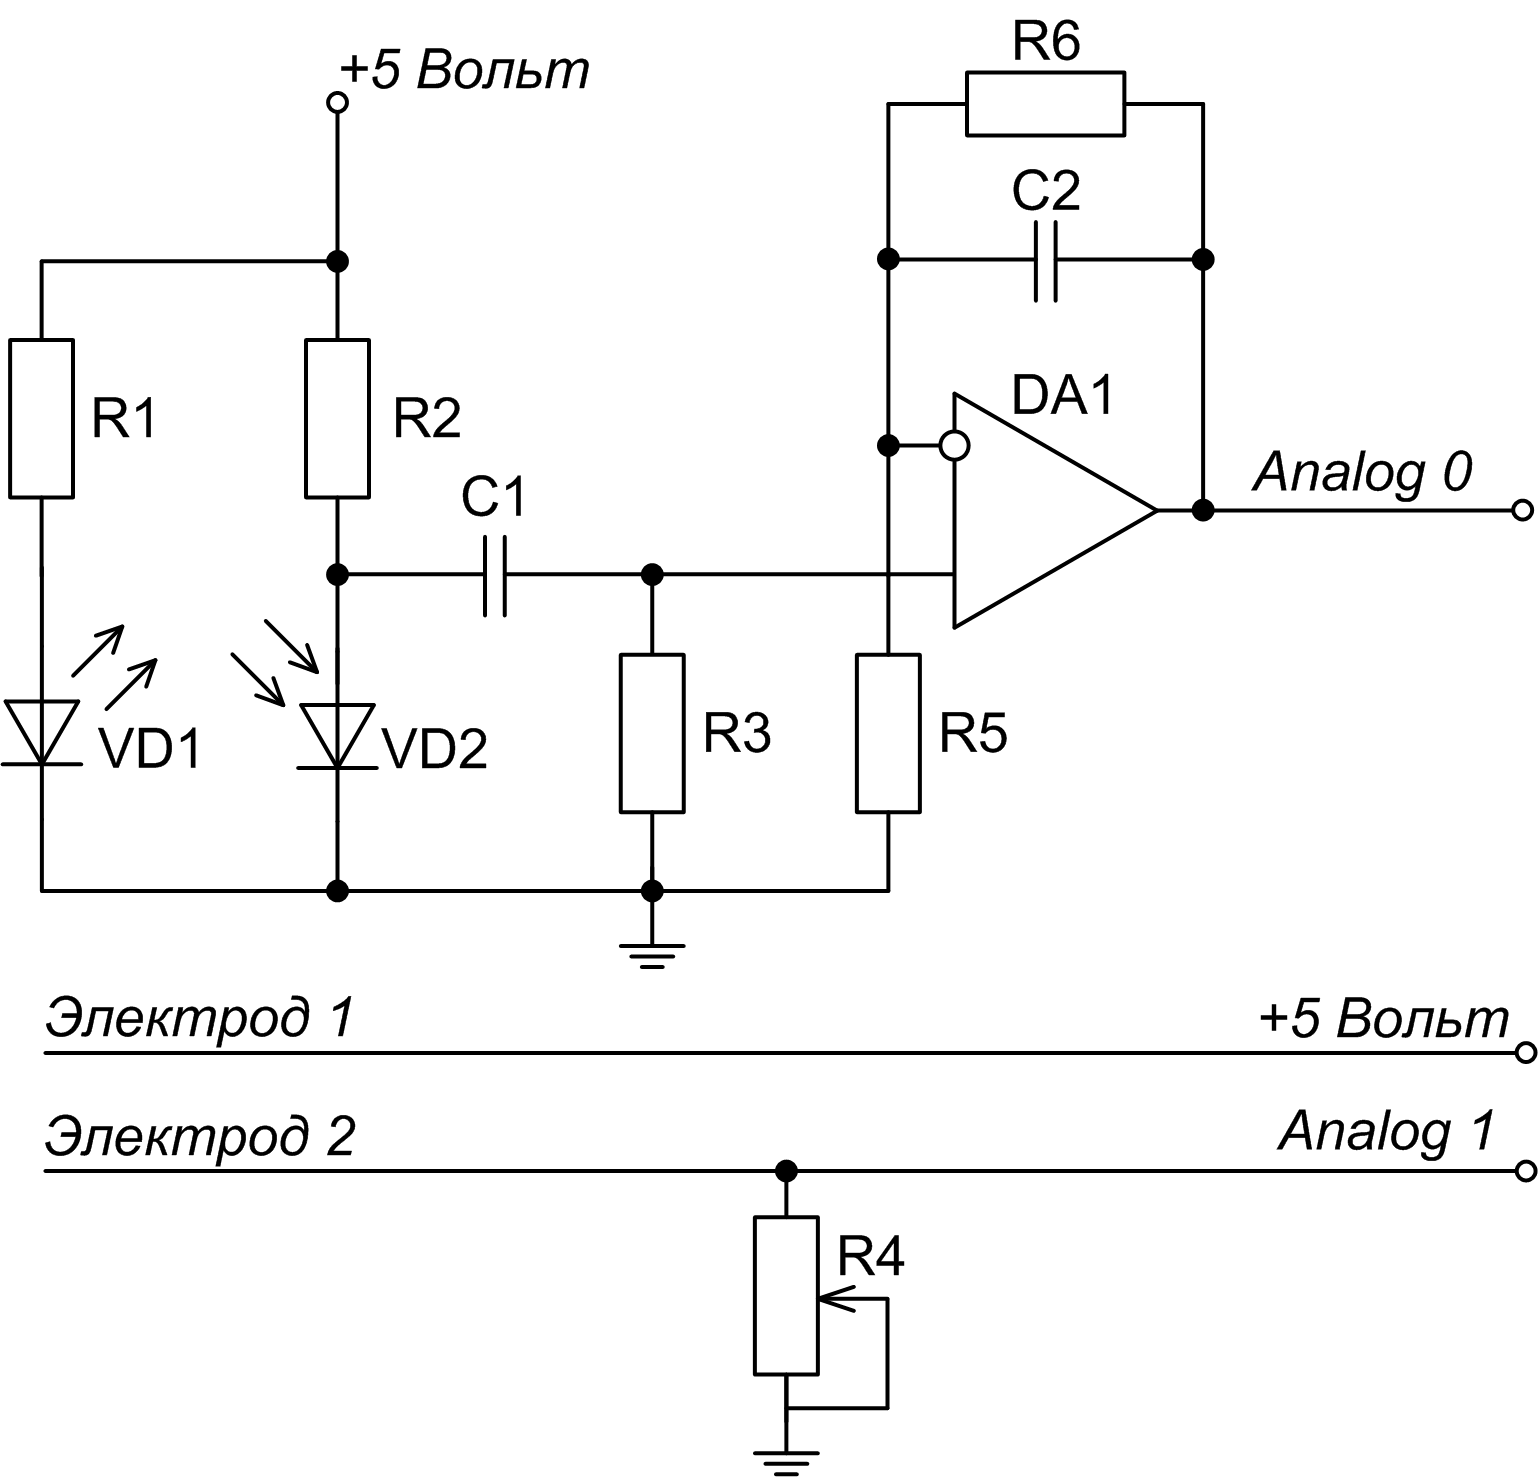
\includegraphics[scale=0.7]{18_2015_fig1}
  \caption{Измерительная подсистема} \label{latij1}
\end{figure}


\begin{figure}[h!]
  \centering 
  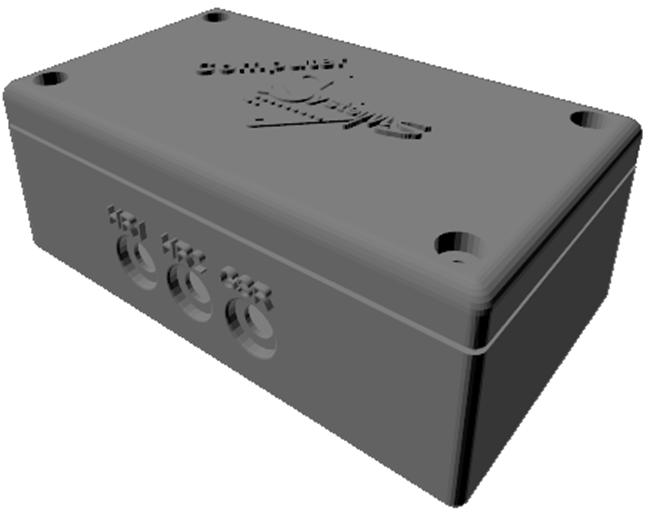
\includegraphics[scale=0.35]{18_2015_fig2} 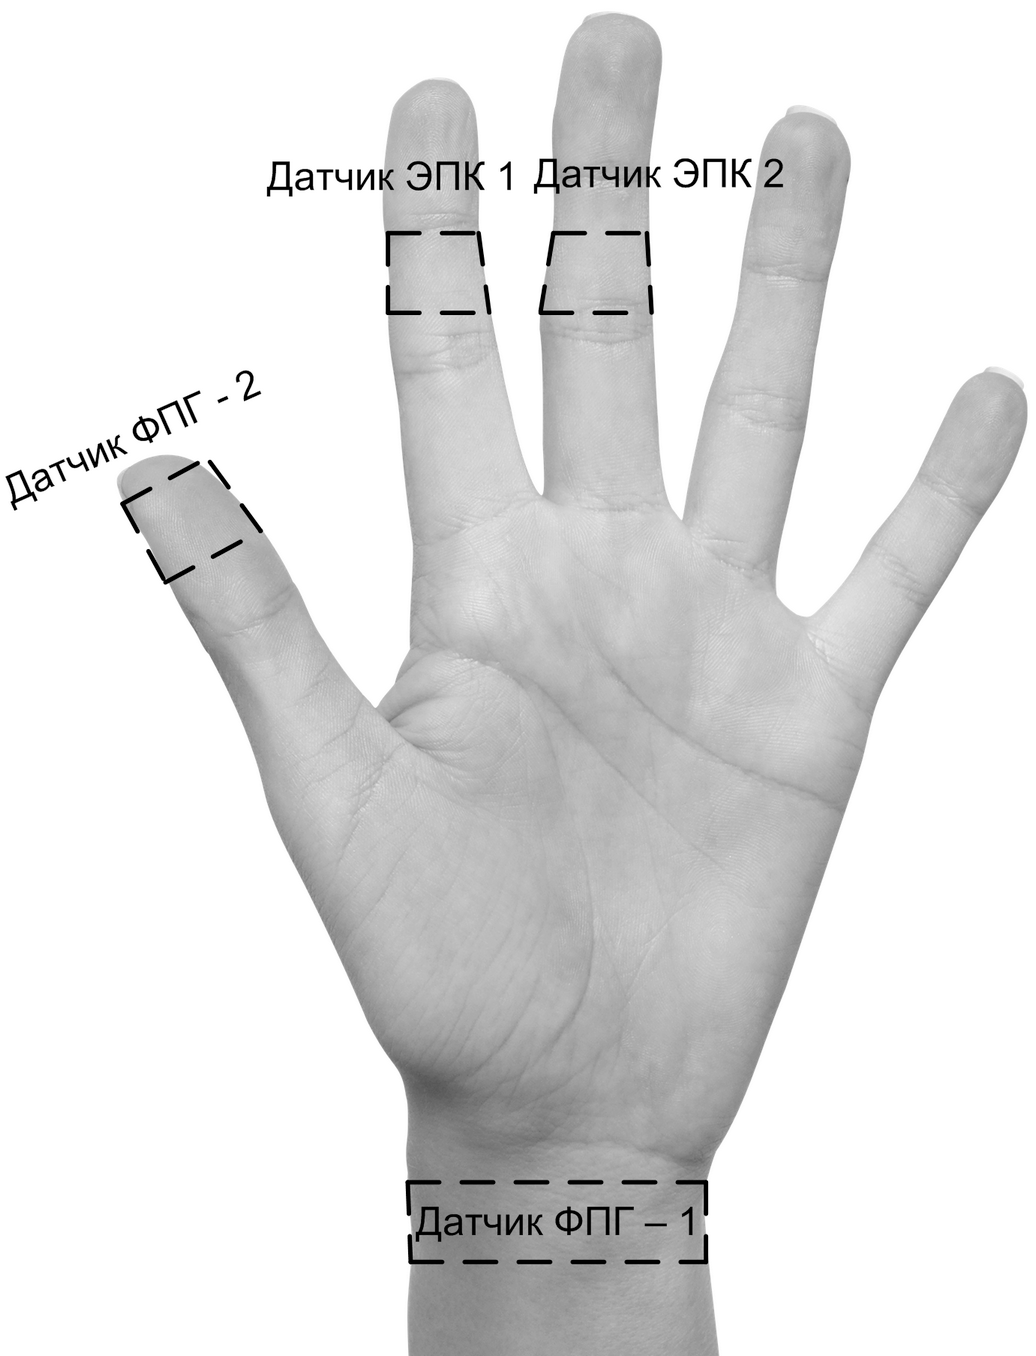
\includegraphics[scale=0.15]{18_2015_fig3} 
  \caption{3D-модель корпуса и схема крепления датчиков} \label{latij2}
\end{figure}

На рисунке \ref{latij2} можно видеть модель для изготовления корпуса устройства методом 3D-печати.

Для подключения щупов (одного для измерения ЭПК, и двух для ЧСС) применяется обычный аудио-разъем 3.5 мм TRS. Для крепления датчиков на текущий момент используются текстильные застёжки (места креплений можно видеть на рисунке \ref{latij2}).

%\begin{figure}[h!]
%  \centering 
%  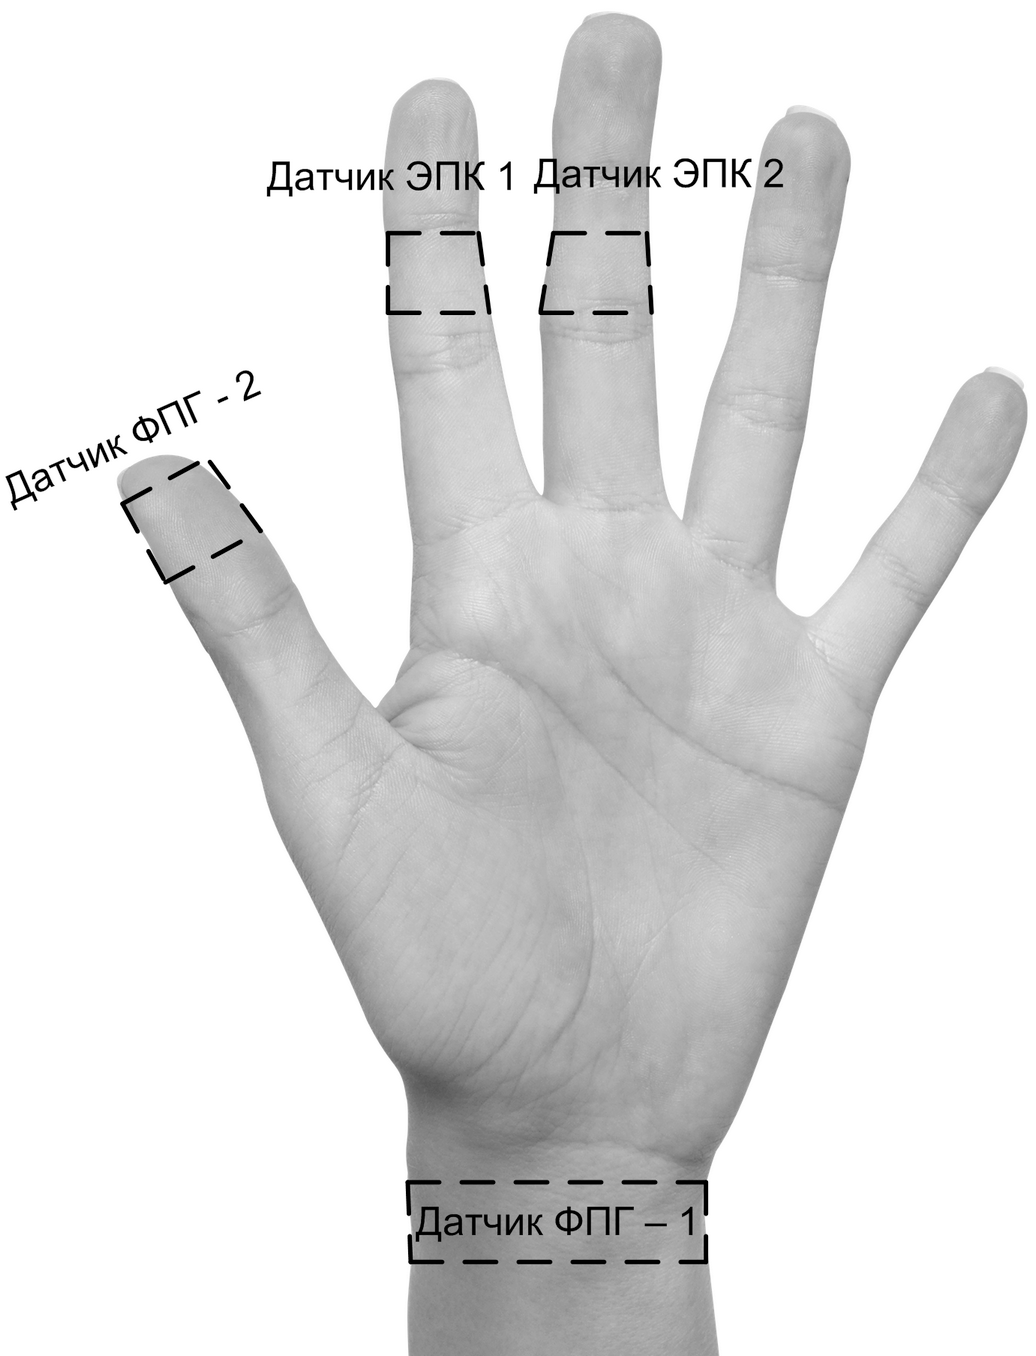
\includegraphics[scale=0.2]{18_2015_fig3} 
%  \caption{Схема крепления датчиков} \label{latij3}
%\end{figure}

Данные передаются в ПК по шине USB, которая одновременно осуществляет питание устройства. Таблица, формируемая принимающим данные ПО, сохраняется в формате CSV для последующего анализа (рисунки \ref{latij4} и \ref{latij5} демонстрируют иллюстративный экран отрисовки снимаемых кривых и фрагмент формируемой таблицы).


\begin{figure}[h!]
  \centering 
  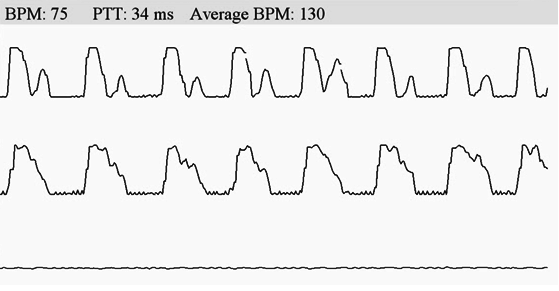
\includegraphics[scale=0.5]{18_2015_fig4}
  \caption{Первичная визуализация средствами processing} \label{latij4}
\end{figure}

\begin{figure}[h!]
  \centering 
  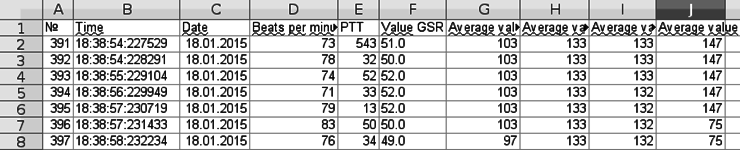
\includegraphics[scale=0.67]{18_2015_fig5}
  \caption{Фрагмент лог-файла} \label{latij5}
\end{figure}

\begin{thebibliography}{9}
\bibitem{bib1} {Kostiuk D.A., Derechennik S.S., Shitikov A.V., Latiy O.O. Approach to evaluate effectiveness of human-computer interaction with contemporary GUI // Третя мiжнародна науково-практична конференцiя FOSS Lviv 2013: Збiрник науковых праць, Львiв, 18–21 квiтня 2013 р. – Львiв, 2013. – С. 85–87.}
\bibitem{bib2} {Лацiй А.А., Касцюк Д.А. Апаратны модуль ацэнкi стану карыстальнiка ПК на базе Arduino // П'ята науково-практична конференцiя FOSS Lviv 2015: Збiрник наукових праць. Львiв, 23–26 квiтня 2015 р. – С. 64–66.}\end{thebibliography}
\end{document}
